

\chapter{Result and Discussion} \label{chap5}
\newpage
\justify
This section presents the implemented interfaces and key functionalities of the MsAdmit system through screenshots captured from the application. Each figure illustrates a specific feature, including student profile intake and resume extraction, applicant dashboard, AI-based university recommendations, semantic university search, SOP evaluation, what-if simulation, and application tracking. Brief descriptions accompany each screenshot to explain its purpose and demonstrate how the system supports students throughout the graduate admission process.
\section{Screenshots of the System}

The visual interfaces and functional screens of the MsAdmit system are presented below with academic figure captions and descriptive explanations.

% Figure 5.1
\begin{figure}[!htbp]
    \centering
    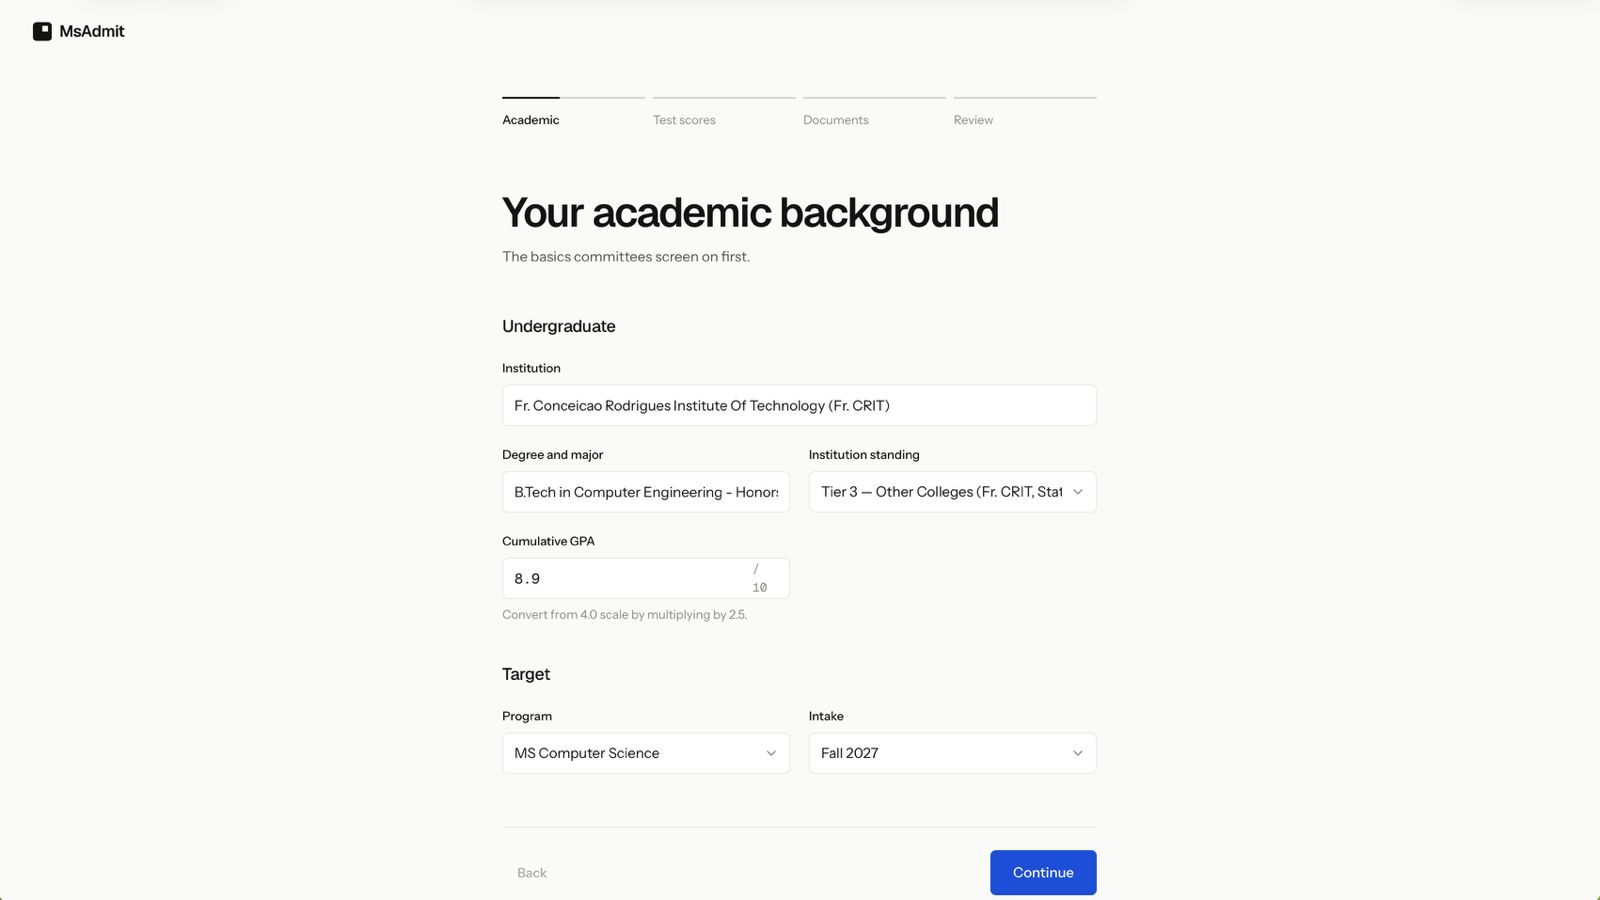
\includegraphics[width=0.85\textwidth]{figure5_1.png}
    \caption{Student Profile Intake \& Resume Extraction Interface}
    \label{fig:profile-intake}

    \vspace{0.2cm}
    \begin{minipage}{0.9\textwidth}
        \small
        Figure~\ref{fig:profile-intake} Displays the initial profile intake interface where applicants can either manually enter academic metrics or upload a PDF resume. The backend extracts relevant work experience (in months), internships, and research papers, automatically populating the form.
    \end{minipage}
\end{figure}

% Figure 5.2
\begin{figure}[!htbp]
    \centering
    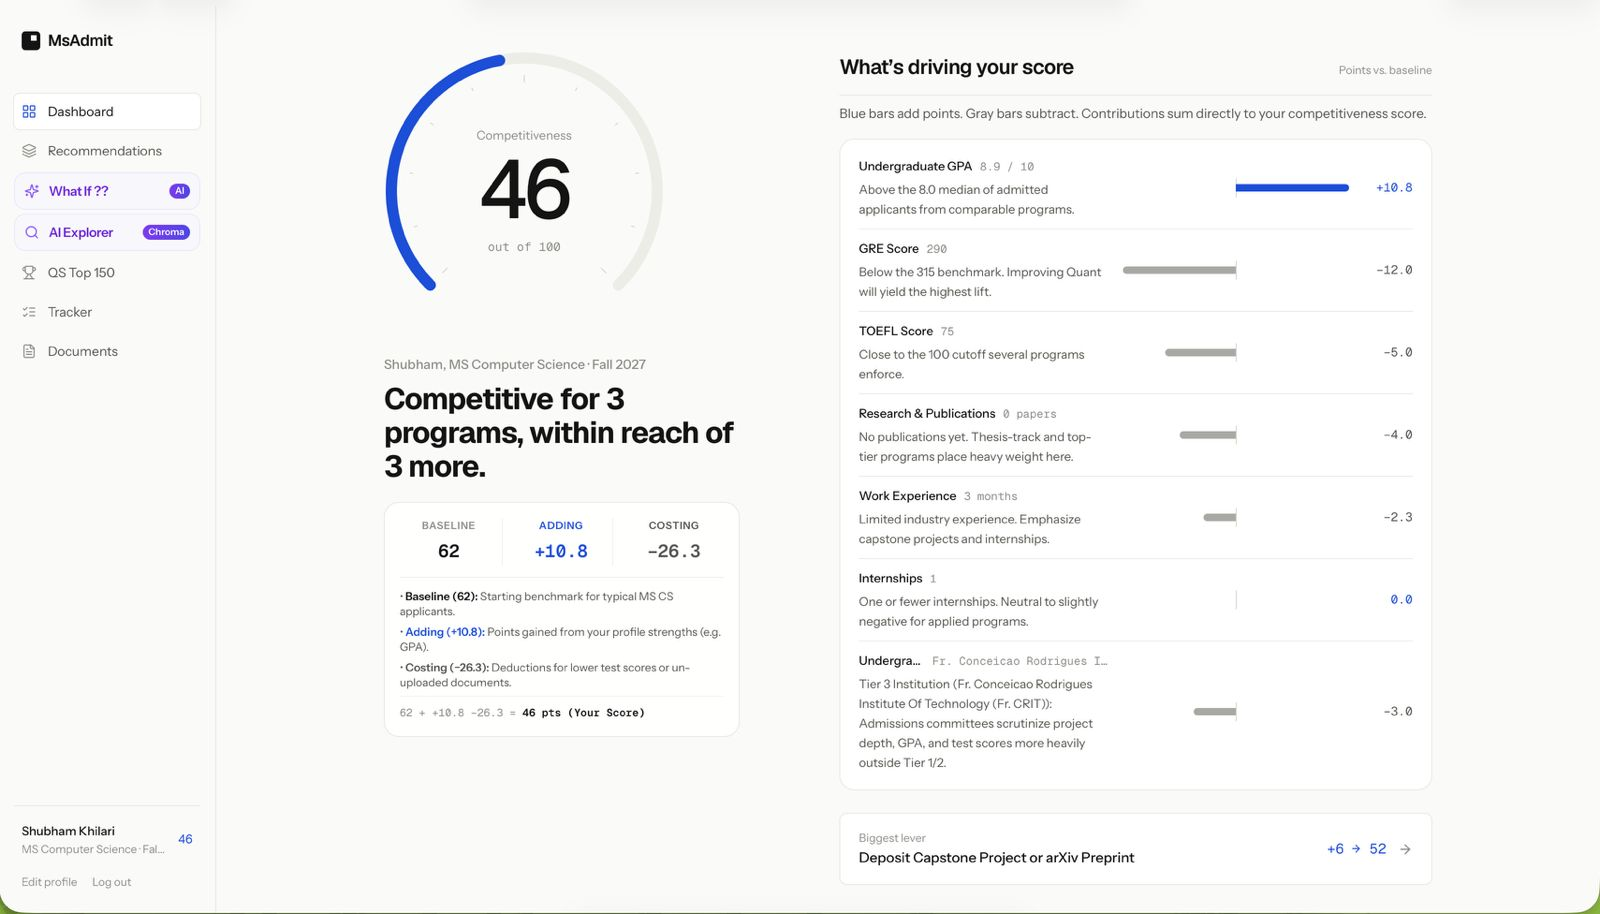
\includegraphics[width=0.85\textwidth]{figure5_2.png}
    \caption{Comprehensive Applicant Dashboard }
    \label{fig:applicant-dashboard}

    \vspace{0.2cm}
    \begin{minipage}{0.9\textwidth}
        \small
        Figure~\ref{fig:applicant-dashboard} Shows the centralized applicant dashboard displaying the calibrated overall Competitiveness Score (0\%--100\%), an alert for the closest upcoming application deadline, an interactive quick-action panel, and a summary breakdown of 3-3-3 university tiers.
    \end{minipage}
\end{figure}

% Figure 5.3
\begin{figure}[!htbp]
    \centering
    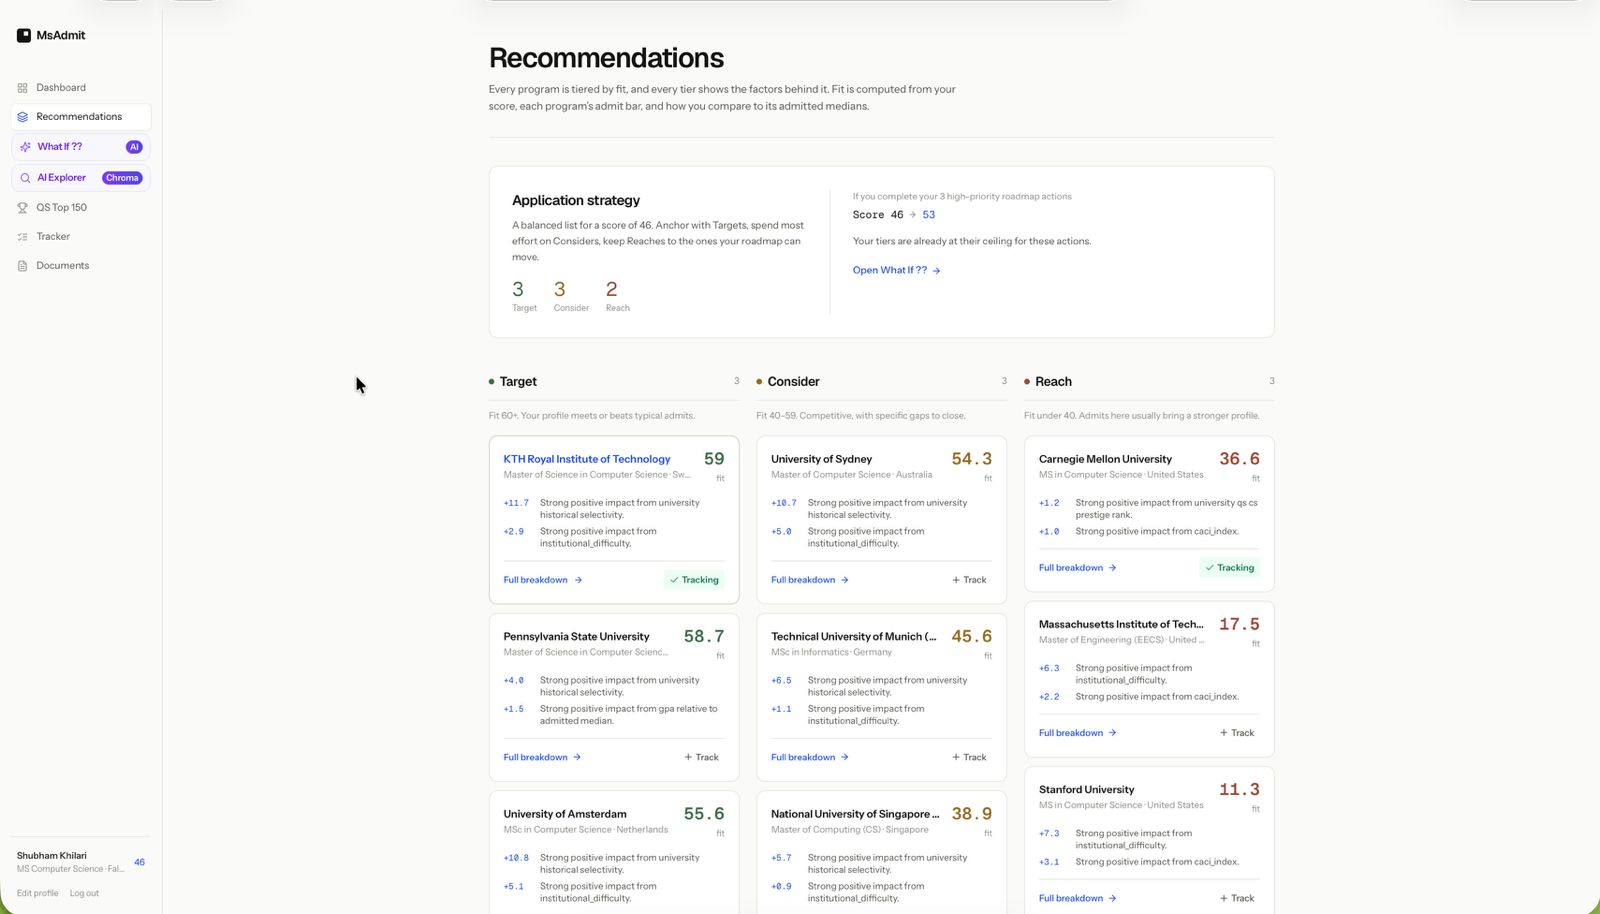
\includegraphics[width=0.85\textwidth]{figure5_3.png}
    \caption{AI University Recommendations with TreeSHAP Explainability Drawer}
    \label{fig:university-recommendations}

    \vspace{0.2cm}
    \begin{minipage}{0.9\textwidth}
        \small
        Figure~\ref{fig:university-recommendations} Demonstrates the recommendation interface displaying categorized Reach, Target, and Consider institution cards. Clicking any university expands the TreeSHAP slide-out drawer, illustrating positive drivers such as strong GPA and publications, along with risk factors such as lower GRE scores or missing work experience.
    \end{minipage}
\end{figure}

% Figure 5.4
\begin{figure}[!htbp]
    \centering
    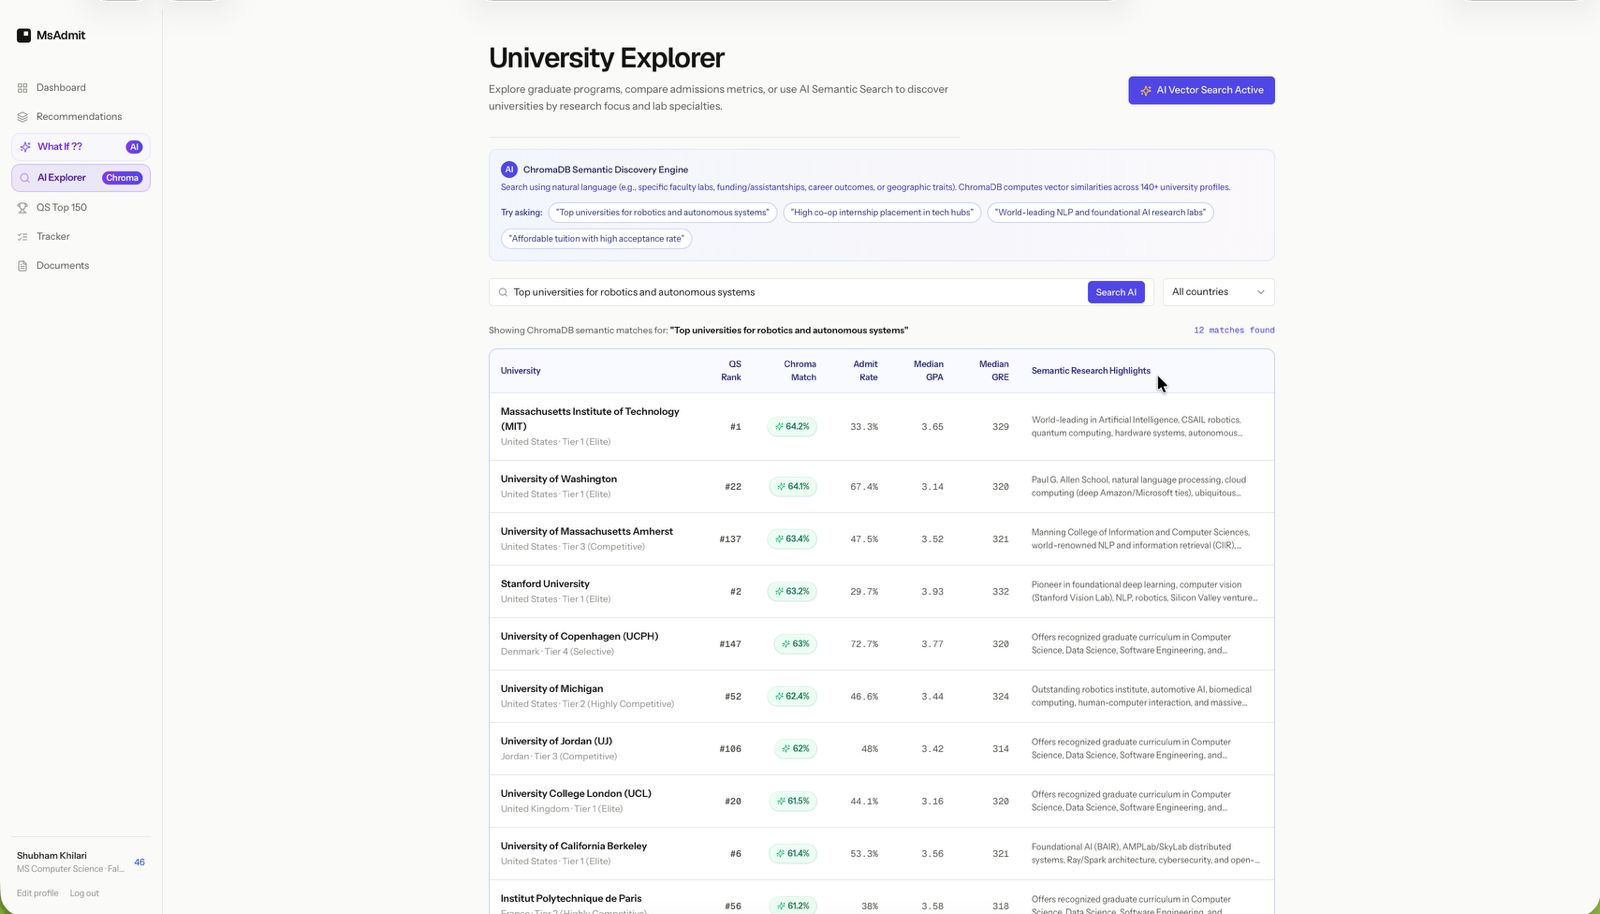
\includegraphics[width=0.85\textwidth]{figure5_4.png}
    \caption{Semantic University Explorer \& Top 150 Rankings Table}
    \label{fig:university-explorer}

    \vspace{0.2cm}
    \begin{minipage}{0.9\textwidth}
        \small
        Figure~\ref{fig:university-explorer} Displays the natural-language semantic search bar powered by ChromaDB. Students can search for research programs, such as AI and robotics with affordable tuition, and explore matching institutions alongside their median admission requirements.
    \end{minipage}
\end{figure}

% Figure 5.5
\begin{figure}[!htbp]
    \centering
    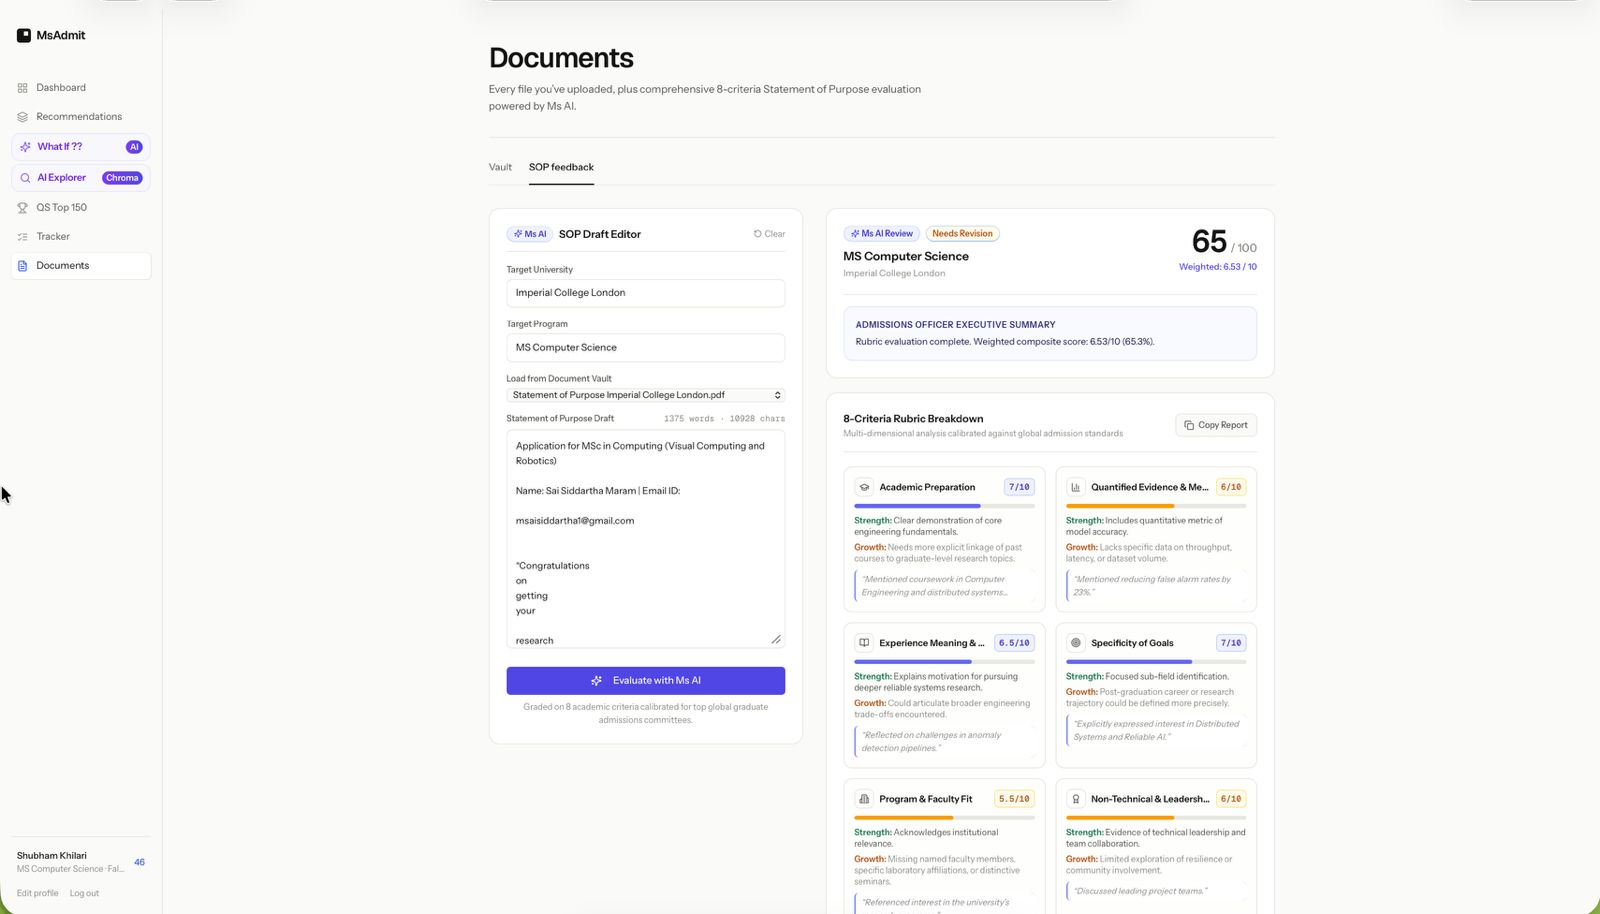
\includegraphics[width=0.85\textwidth]{figure5_5.png}
    \caption{Document Vault \& Gemini 1.5 8-Criteria SOP Evaluation Interface}
    \label{fig:document-vault}

    \vspace{0.2cm}
    \begin{minipage}{0.9\textwidth}
        \small
        Figure~\ref{fig:document-vault} Displays the document evaluation workspace showing an uploaded Statement of Purpose, a radar or progress breakdown across the eight criteria, and paragraph-by-paragraph revision suggestions.
    \end{minipage}
\end{figure}

% Figure 5.6
\begin{figure}[!htbp]
    \centering
    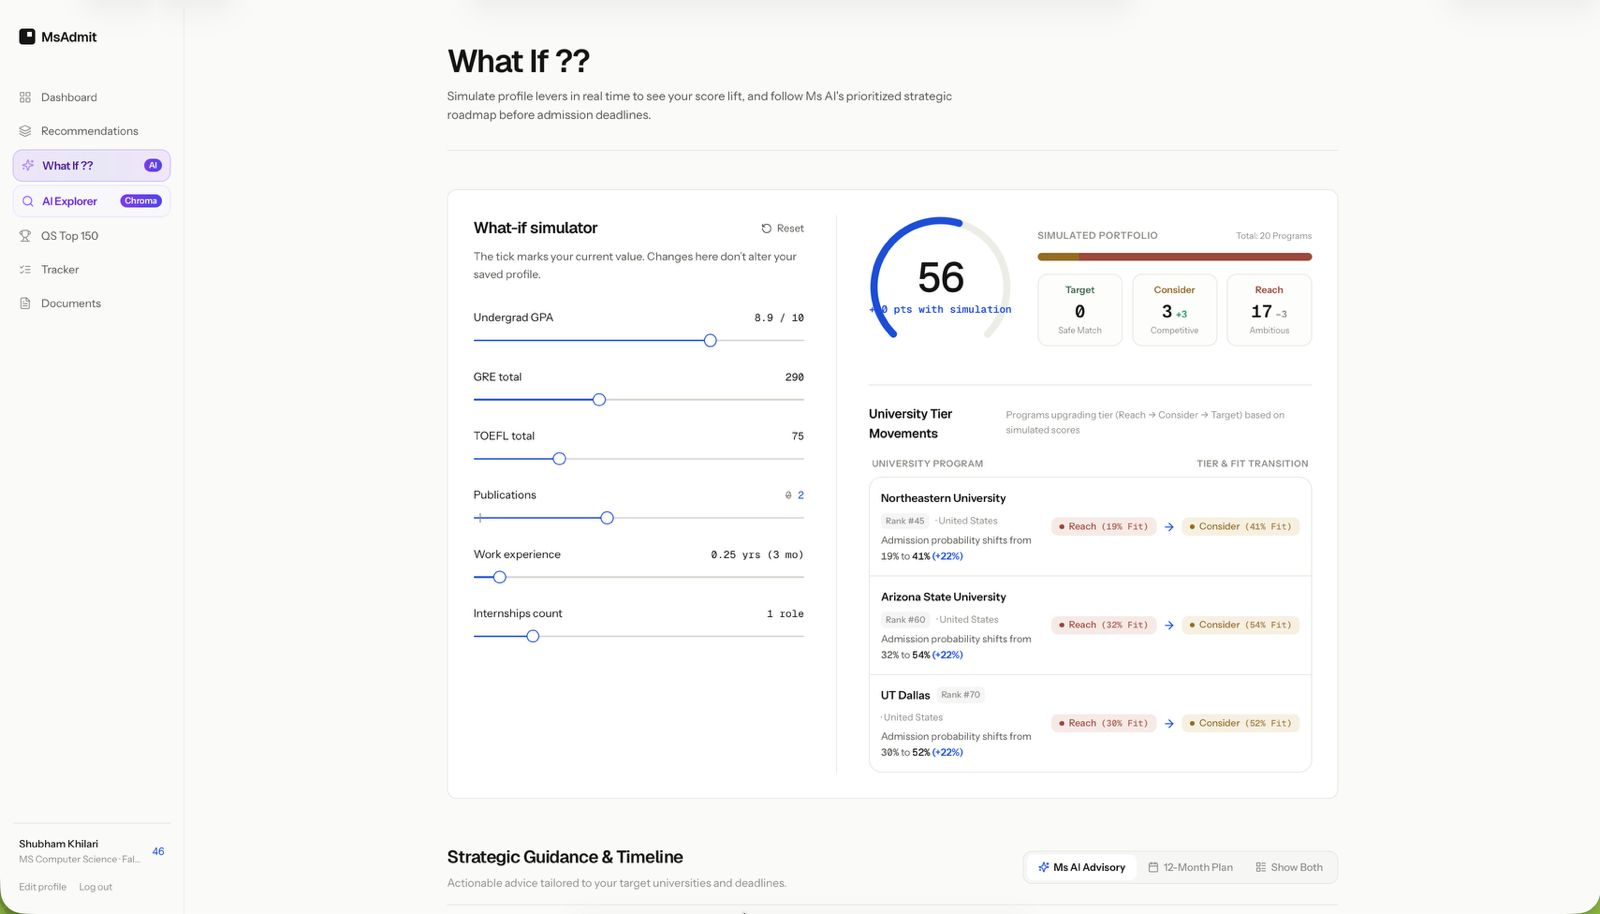
\includegraphics[width=0.85\textwidth]{figure5_6.png}
    \caption{Interactive What-If Simulator \& Dynamic Optimization Roadmap}
    \label{fig:optimization-roadmap}

    \vspace{0.2cm}
    \begin{minipage}{0.9\textwidth}
        \small
        Figure~\ref{fig:optimization-roadmap} Illustrates the What-If simulation workspace where students can adjust GRE Quantitative and Verbal scores, GPA, and research publications to observe real-time recalculations of admission probabilities and updated university tier classifications.
    \end{minipage}
\end{figure}

% Figure 5.7
\begin{figure}[!htbp]
    \centering
    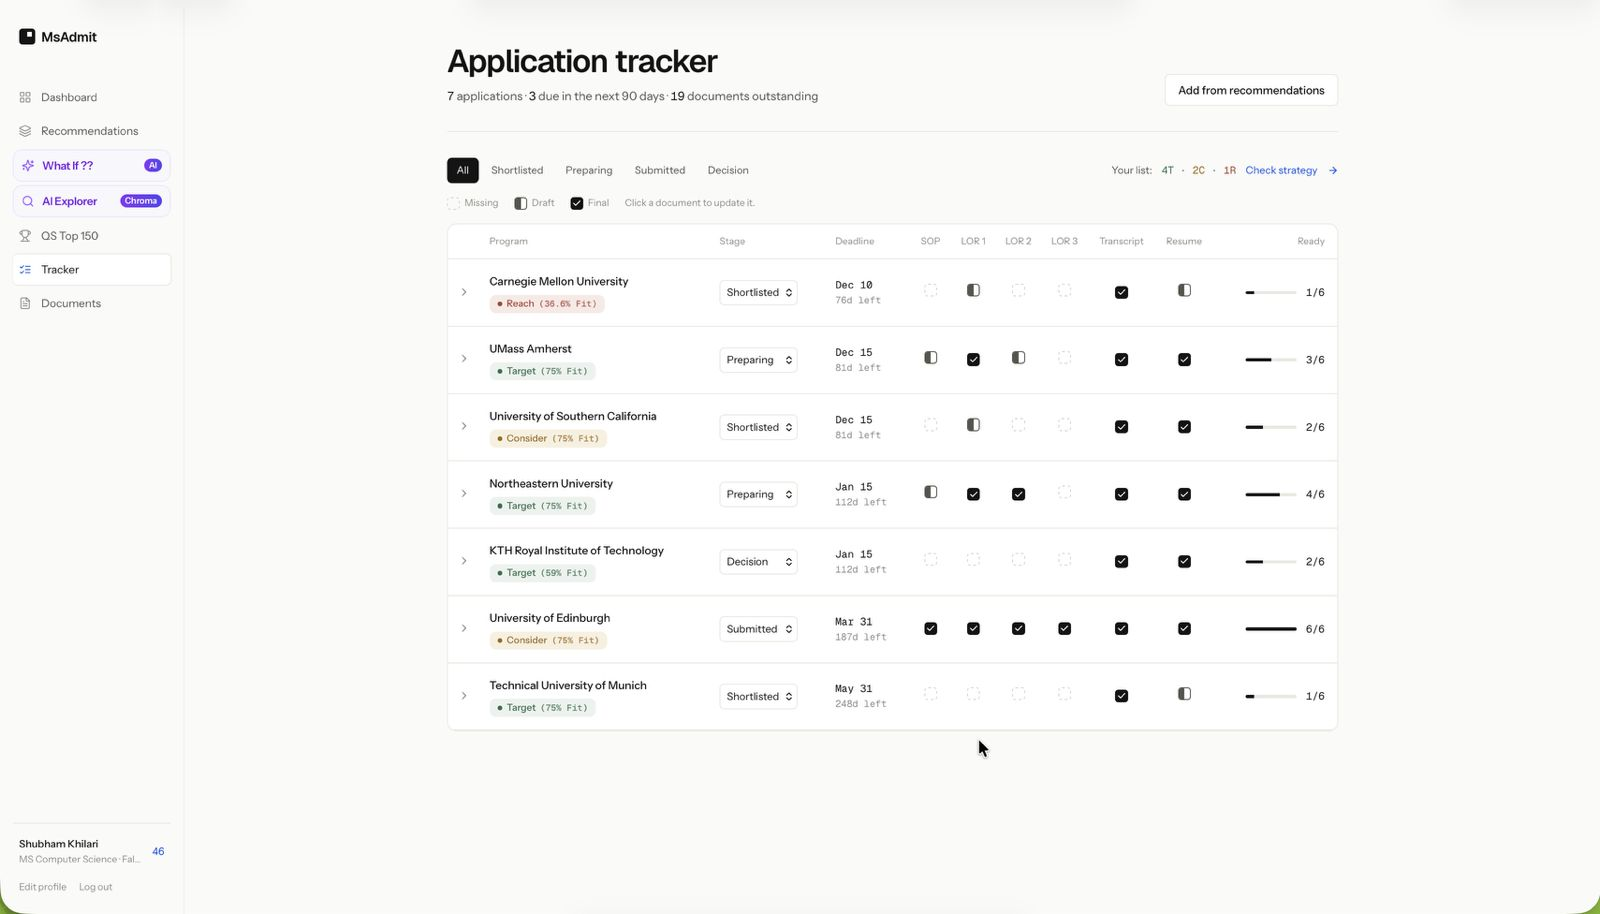
\includegraphics[width=0.85\textwidth]{figure5_7.png}
    \caption{Active Application Tracker \& Document Progress Workspace}
    \label{fig:application-tracker}

    \vspace{0.2cm}
    \begin{minipage}{0.9\textwidth}
        \small
        Figure~\ref{fig:application-tracker} Highlights the application management tracker showing shortlisted programs, a six-stage document checklist (SOP, LOR 1--3, transcripts, and resume), a deadline countdown, and a cumulative application fee budget calculator.
    \end{minipage}
\end{figure}

\clearpage


\section{Sample Code (Key Algorithms \& Core Logic)}

%--------------------------------------------------
% Listing 5.1
%--------------------------------------------------
\subsection{Multi-Model Stacking Ensemble Training and Calibration}

\begin{lstlisting}[language=Python]
from lightgbm import LGBMClassifier
from xgboost import XGBClassifier
from sklearn.ensemble import (
    ExtraTreesClassifier,
    RandomForestClassifier,
    StackingClassifier
)
from sklearn.linear_model import LogisticRegression

def build_stacking_ensemble(X_train, y_train):
    estimators = [
        ('xgb', XGBClassifier(
            n_estimators=300,
            learning_rate=0.025,
            max_depth=6,
            subsample=0.85,
            colsample_bytree=0.85,
            random_state=42
        )),
        ('lgbm', LGBMClassifier(
            n_estimators=300,
            learning_rate=0.03,
            max_depth=6,
            num_leaves=15,
            random_state=42
        )),
        ('rf', RandomForestClassifier(
            n_estimators=150,
            max_depth=14,
            min_samples_leaf=3,
            random_state=42
        )),
        ('et', ExtraTreesClassifier(
            n_estimators=150,
            max_depth=14,
            min_samples_leaf=3,
            random_state=42
        ))
    ]

    stacking_classifier = StackingClassifier(
        estimators=estimators,
        final_estimator=LogisticRegression(
            C=1.0,
            max_iter=500,
            random_state=42
        ),
        cv=5,
        n_jobs=-1,
        passthrough=False
    )

    stacking_classifier.fit(X_train, y_train)
    return stacking_classifier
\end{lstlisting}
This code builds and trains a stacking ensemble classifier that combines XGBoost, LightGBM, Random Forest, and Extra Trees, using Logistic Regression as the meta-classifier to predict admission outcomes.


%--------------------------------------------------
% Listing 5.2
%--------------------------------------------------
\clearpage
\subsection{Admission Prediction and TreeSHAP Attribution Logic}

\begin{lstlisting}[language=Python]
from typing import Dict, Any

def compute_prediction_and_shap(
    profile_input: Dict[str, Any]
) -> Dict[str, Any]:
    """Calculate admission score and profile contributions."""

    engine = get_ml_engine()
    normalized = normalize_profile(profile_input)

    portfolio = engine.recommend_portfolio(
        normalized,
        top_k=3,
        include_shap=True
    )

    gpa = normalized["gpa"]
    gre = normalized["gre"]
    pubs = normalized["research_publications"]
    work_months = int(
        profile_input.get("work_months", 0)
    )

    def clamp(v: float, lo: float, hi: float) -> float:
        return max(lo, min(hi, v))

    gpa_contrib = round(
        clamp((gpa - 8.0) * 12.0, -12.0, 12.0), 1
    )
    gre_contrib = round(
        (gre - 315.0) * 0.9, 1
    )
    research_contrib = round(
        min(10.0, pubs * 3.5), 1
    )
    work_contrib = round(
        min(7.0, work_months / 36.0 * 8.0), 1
    )

    return {
        "overall_score": portfolio.get(
            "overall", 72.0
        ),
        "portfolio": portfolio.get("universities", []),
        "gpa_contribution": gpa_contrib,
        "gre_contribution": gre_contrib,
        "research_contribution": research_contrib,
        "work_contribution": work_contrib
    }
\end{lstlisting}
This function calculates an applicant’s overall admission score, recommends the top three universities, and estimates the individual contributions of GPA, GRE, research publications, and work experience to their profile.

%--------------------------------------------------
% Listing 5.3
%--------------------------------------------------
\clearpage
\subsection{Statement of Purpose Evaluation Using Gemini}

\begin{lstlisting}[language=Python]
import json
import google.generativeai as genai

def evaluate_sop_against_rubric(
    sop_text: str,
    target_university: str
):
    """Evaluate an SOP against eight criteria."""

    prompt = f"""
    Evaluate the following Statement of Purpose for
    {target_university}.

    Score the SOP on eight criteria:
    1. Academic motivation
    2. Program fit
    3. Research interests
    4. Relevant experience
    5. Career goals
    6. Specificity
    7. Structure and clarity
    8. Grammar and writing quality

    Return a JSON object containing scores and
    actionable feedback for each criterion.

    Statement of Purpose:
    {sop_text}
    """

    model = genai.GenerativeModel(
        "gemini-1.5-flash"
    )
    response = model.generate_content(prompt)

    result = json.loads(response.text.strip())
    return result
\end{lstlisting}

\vspace{25pt}
This function uses Google Gemini 1.5 Flash to evaluate a Statement of Purpose against eight criteria, returning a JSON object containing scores and actionable feedback for each criterion.



%--------------------------------------------------
% Listing 5.4
%--------------------------------------------------
\clearpage
\subsection{Semantic University Retrieval Using ChromaDB}

\begin{lstlisting}[language=Python]
import chromadb

class ChromaService:
    def __init__(self, persist_directory: str):
        self.client = chromadb.PersistentClient(
            path=persist_directory
        )

        self.collection = self.client.get_or_create_collection(
            name="universities_semantic_catalog",
            metadata={"hnsw:space": "cosine"}
        )

    def search_universities(
        self,
        query_embedding,
        top_k: int = 10
    ):
        results = self.collection.query(
            query_embeddings=[query_embedding],
            n_results=top_k
        )

        matches = []

        distances = results.get("distances", [[]])[0]
        ids = results.get("ids", [[]])[0]
        documents = results.get("documents", [[]])[0]
        metadatas = results.get("metadatas", [[]])[0]

        for i, dist in enumerate(distances):
            matches.append({
                "id": ids[i],
                "document": documents[i],
                "metadata": metadatas[i],
                "similarity": 1.0 - dist
            })

        return matches
\end{lstlisting}

\vspace{25pt}

This code implements a ChromaDB-based semantic search service that retrieves the top matching universities using embedding similarity and returns their IDs, documents, metadata, and similarity scores.


%--------------------------------------------------
% Listing 5.5
%--------------------------------------------------
\clearpage
\subsection{Hybrid In-Memory Cache with TTL Fallback}

\begin{lstlisting}[language=Python]
import time
import threading

class SafeInMemoryCache:
    def __init__(self, default_ttl: int = 300):
        self.store = {}
        self.lock = threading.Lock()
        self.default_ttl = default_ttl

    def get(self, key):
        with self.lock:
            item = self.store.get(key)

            if item is None:
                return None

            value, expiry = item

            if time.time() >= expiry:
                del self.store[key]
                return None

            return value

    def set(self, key, value, ttl=None):
        if ttl is None:
            ttl = self.default_ttl

        expiry = time.time() + ttl

        with self.lock:
            self.store[key] = (value, expiry)

    def delete(self, key):
        with self.lock:
            self.store.pop(key, None)

    def clear(self):
        with self.lock:
            self.store.clear()
\end{lstlisting}
\vspace{25p}
This code implements a thread-safe in-memory cache with TTL (Time To Live) that stores key-value pairs temporarily, automatically removes expired entries, and supports retrieving, setting, deleting, and clearing cached data.

\clearpage

\section{Testing}

A rigorous three-tier verification pyramid comprising
\textbf{Unit Testing, Integration Testing, and Blackbox Testing} was
executed to validate system accuracy, numerical stability, API security,
and fault tolerance.

%==================================================
% 5.3.1 UNIT TESTING -- OWN PAGE
%==================================================

\subsection{Unit Testing}

\begingroup
\small
\setlength{\tabcolsep}{4pt}
\renewcommand{\arraystretch}{1.4}



\begin{table}[htbp]
\centering
\caption{Unit Testing Results for the MsAdmit System}
\label{tab:unit-testing}

\normalsize
\renewcommand{\arraystretch}{1.7}
\setlength{\tabcolsep}{6pt}

\begin{tabularx}{\textwidth}{
|>{\centering\arraybackslash}p{1.0cm}
|>{\raggedright\arraybackslash}X
|>{\raggedright\arraybackslash}X
|>{\raggedright\arraybackslash}X
|>{\raggedright\arraybackslash}X
|>{\centering\arraybackslash}p{1.2cm}|}
\hline
\textbf{Test ID} &
\textbf{Module / Function} &
\textbf{Input Test Data} &
\textbf{Expected Output} &
\textbf{Actual Result} &
\textbf{Status} \\
\hline

UT-01 &
\makecell[l]{\texttt{normalize\_}\\\texttt{profile()}} &
Indian CGPA = 8.8 / 10.0 &
Scaled GPA = 3.52 / 4.0 &
Scaled GPA = 3.52 &
PASS \\
\hline

UT-02 &
\makecell[l]{\texttt{normalize\_}\\\texttt{profile()}} &
Standard US GPA = 3.75 &
Unchanged GPA = 3.75 &
GPA = 3.75 &
PASS \\
\hline

UT-03 &
TreeSHAP Clamping &
Outlier GRE = 340 &
Contribution capped at +12.0\% &
Contribution = +12.0\% &
PASS \\
\hline

UT-04 &
\makecell[l]{\texttt{extract\_text\_}\\\texttt{from\_pdf()}} &
2-page resume PDF &
Extracted string $\geq$ 500 chars &
Extracted 1,420 chars &
PASS \\
\hline

UT-05 &
\makecell[l]{SafeInMemory\\Cache} &
Key set TTL = 1s; read at 1.5s &
Expired, returns None &
Returned None &
PASS \\
\hline

UT-06 &
\makecell[l]{\texttt{CRITERIA\_}\\\texttt{WEIGHTS}} &
Sum of 8 criteria weights &
Exact cumulative sum = 1.00 &
Sum = 1.0000 &
PASS \\
\hline

\end{tabularx}
\end{table}



The Table 5.1 shows  unit testing results demonstrate that all six test cases passed.
The tests verified GPA normalization, TreeSHAP contribution clamping,
PDF text extraction, cache expiration, and SOP evaluation criteria
weight validation. These results indicate that the tested components
performed as expected under the specified test conditions.

\endgroup


%==================================================
% 5.3.2 INTEGRATION TESTING -- OWN PAGE
%==================================================
\clearpage
\subsection{Integration Testing}

\begingroup
\small
\setlength{\tabcolsep}{3pt}
\renewcommand{\arraystretch}{1.35}



\begin{table}[htbp]
\centering
\caption{Integration Testing Results for the MsAdmit System}
\label{tab:integration-testing}

\normalsize
\setlength{\tabcolsep}{5pt}
\renewcommand{\arraystretch}{1.6}

\begin{tabularx}{\textwidth}{
|>{\centering\arraybackslash}p{1.0cm}
|>{\raggedright\arraybackslash}X
|>{\raggedright\arraybackslash}X
|>{\raggedright\arraybackslash}X
|>{\raggedright\arraybackslash}X
|>{\centering\arraybackslash}p{1.2cm}|}
\hline
\textbf{Test ID} &
\textbf{Subsystems Tested} &
\textbf{Execution Flow} &
\textbf{Expected Behavior} &
\textbf{Actual Result} &
\textbf{Status} \\
\hline

IT-01 &
Client $\rightarrow$ API $\rightarrow$ DB &
\texttt{/auth/signup} &
User created, password hashed, JWT returned &
Status 201; JWT verified &
PASS \\
\hline

IT-02 &
Client $\rightarrow$ Predict $\rightarrow$ ML &
\texttt{/predict} &
Ensemble generates 3-3-3 tiers &
Score and 9 universities returned &
PASS \\
\hline

IT-03 &
Router $\rightarrow$ Redis Cache &
Duplicate \texttt{/predict} &
Cached response in $<$10 ms &
Cache hit; latency 4.2 ms &
PASS \\
\hline

IT-04 &
Docs $\rightarrow$ PyPDF $\rightarrow$ Gemini &
\texttt{/documents/evaluate} &
Text extracted; 8 scores returned in JSON &
8 criteria scores and feedback returned &
PASS \\
\hline

IT-05 &
Explorer $\rightarrow$ ChromaDB &
\texttt{/search} &
Matching universities ranked &
6 ranked universities with scores &
PASS \\
\hline

IT-06 &
Tracker $\rightarrow$ MongoDB &
\texttt{PATCH /profile} &
Checklist update persisted &
Application record updated &
PASS \\
\hline

\end{tabularx}
\end{table}

\vspace{25pt}


The Table 5.2 shows All six integration tests passed, validating communication among
the client, API, database, Machine Learning model, Redis cache,
document evaluation module, ChromaDB search subsystem, and
MongoDB application tracker.

\endgroup



%==================================================
% 5.3.3 BLACKBOX TESTING -- OWN PAGE
%==================================================
\clearpage
\subsection{Blackbox Testing}

\begingroup
\small
\setlength{\tabcolsep}{4pt}
\renewcommand{\arraystretch}{1.4}



\begin{table}[htbp]
\centering
\caption{Blackbox Testing Results for the MsAdmit System}
\label{tab:blackbox-testing}

\normalsize
\setlength{\tabcolsep}{5pt}
\renewcommand{\arraystretch}{1.6}

\begin{tabularx}{\textwidth}{
|>{\centering\arraybackslash}p{1.0cm}
|>{\raggedright\arraybackslash}X
|>{\raggedright\arraybackslash}X
|>{\raggedright\arraybackslash}X
|>{\raggedright\arraybackslash}X
|>{\centering\arraybackslash}p{1.2cm}|}
\hline
\textbf{Test ID} &
\textbf{Scenario / Feature} &
\textbf{User Input / Action} &
\textbf{Expected Behavior} &
\textbf{Actual Result} &
\textbf{Status} \\
\hline

BT-01 &
Auth Boundary &
Login with unregistered email &
Display invalid credentials (401) &
Alert displayed; access denied &
PASS \\
\hline

BT-02 &
GRE Boundary &
Enter GRE = 350 ($>$ 340) &
Prevent form submission &
Error: GRE must be 260--340 &
PASS \\
\hline

BT-03 &
GPA Boundary &
Enter GPA = 0.0 &
Highlight invalid input &
Submission blocked; GPA must be $>$ 0 &
PASS \\
\hline

BT-04 &
Invalid File Format &
Upload .exe or .png as SOP &
Reject non-PDF files &
File rejected immediately &
PASS \\
\hline

BT-05 &
Empty PDF SOP &
Upload blank PDF &
Notify user of unreadable text &
Warning displayed; no crash &
PASS \\
\hline

BT-06 &
What-If Simulator &
Move GRE slider from 310 to 325 &
Recalculate score and tier &
Probability changes by +8.5\%; tiers updated &
PASS \\
\hline

BT-07 &
Session Expiry &
Open dashboard with expired JWT &
Clear token and redirect to login &
Redirects to login screen &
PASS \\
\hline

\end{tabularx}
\end{table}
\vspace{25pt}

The Table 5.3 shows All seven blackbox tests passed, validating authentication,
input boundary checks, file-upload validation, empty-document
handling, real-time profile simulation, and session-expiry
management. The results indicate that the tested features
responded as expected to the specified user inputs.

\endgroup

\clearpage

\newpage


\subsection{Machine Learning Architecture \& Predictive Modeling Pipeline}

A two-tier stacking ensemble is designed using
\texttt{StackingClassifier}. The base learners (Level 0)
generate out-of-fold probabilistic predictions using
five-fold cross-validation (CV = 5). These predictions are
then passed to a Level-1 Logistic Regression meta-classifier.

\begin{figure}[!htbp]
    \centering
    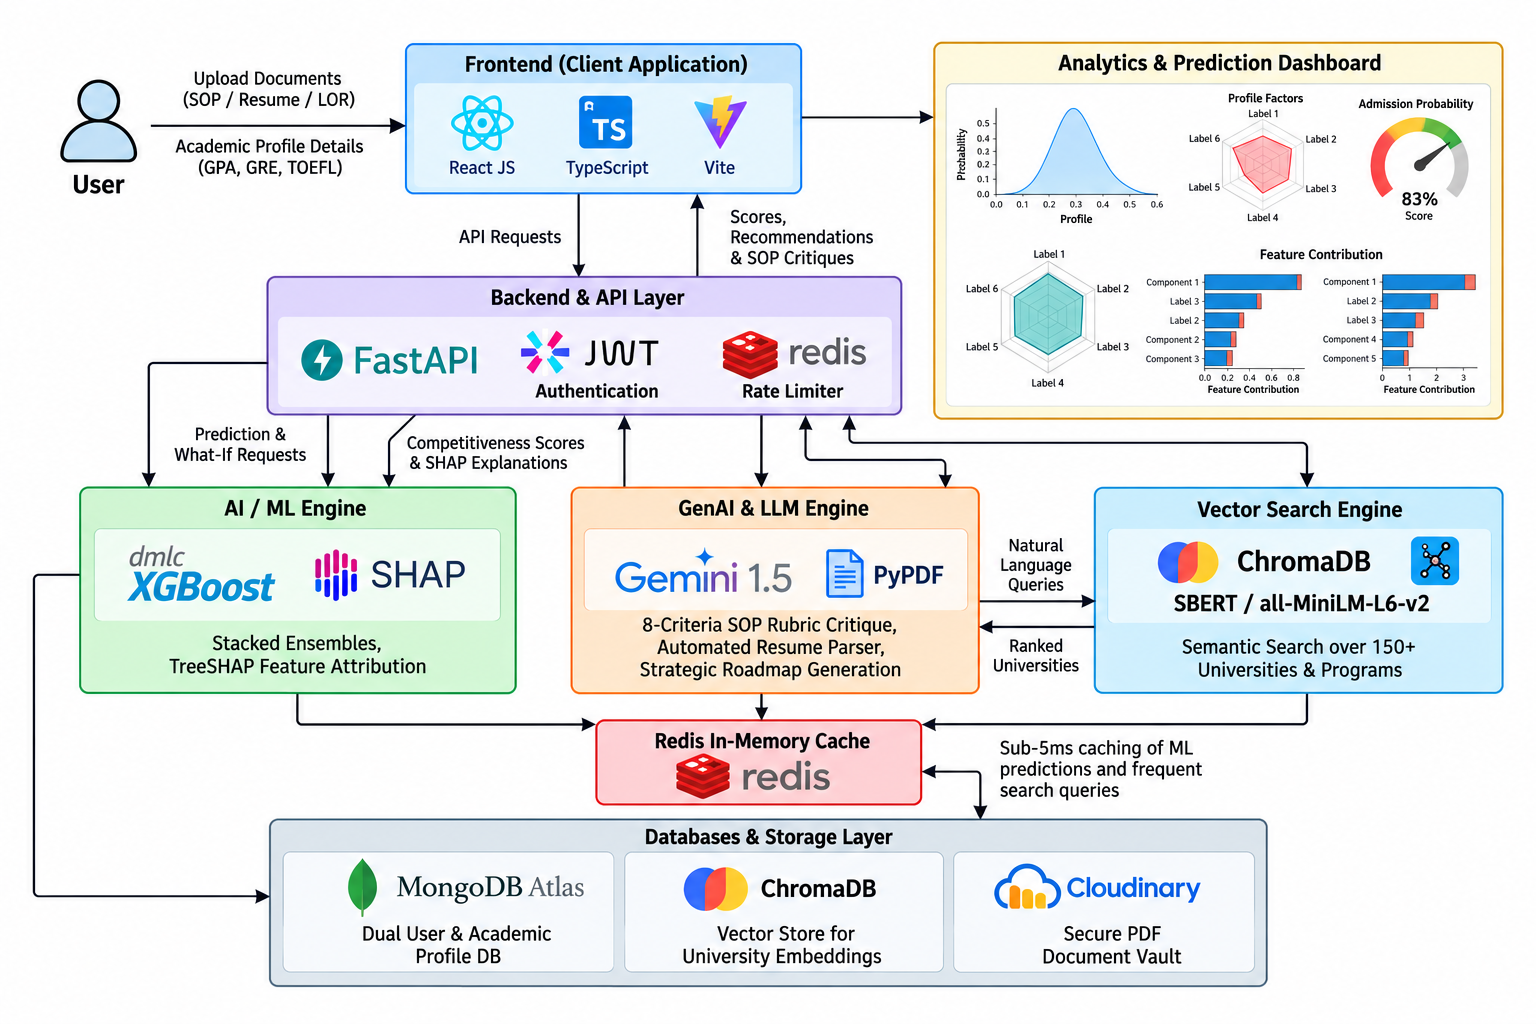
\includegraphics[width=\columnwidth]{System_Arch.png}
    \caption{ML Model Architecture: Ensemble Stacking and Explainability}
    \label{fig:ml_model_architecture}
\end{figure}

Figure~\ref{fig:ml_model_architecture} illustrates the ensemble 
stacking architecture of the proposed admission prediction model, 
integrating four base classifiers with five-fold cross-validation 
and a Logistic Regression meta-classifier to predict admission 
probabilities. SHAP TreeExplainer provides feature attribution 
values, improving the interpretability and transparency of the 
model's predictions.




%------------------------------------------------
% Comparative Model Evaluation
%------------------------------------------------

\subsection{Comparative Model Performance Evaluation}

All candidate models were evaluated on the held-out test set
($N = 11{,}655$) using ROC-AUC, accuracy, precision, recall,
F1-score, and Brier score. These metrics assess classification
performance and probabilistic prediction quality. A lower Brier
score indicates better probabilistic accuracy.



%------------------------------------------------
% Discussion and Key Observations
%------------------------------------------------

\subsection{Discussion and Key Observations}

\begin{enumerate}

    \item \textbf{Superior Overall Performance:}
    The stacking ensemble achieved the highest ROC-AUC of 0.8465,
    outperforming XGBoost (0.8418) and the Logistic Regression
    baseline (0.7412). Its accuracy of 76.26\% and F1-score of
    0.7896 further support its selection as the production model.

    \item \textbf{Recall and Applicant Guidance:}
    The ensemble achieved a recall of 0.8130 (81.30\%), indicating
    that it identified a substantial proportion of positive cases
    in the test set. Recall is relevant because false-negative
    predictions may cause applicants to overlook potentially
    suitable opportunities.

    \item \textbf{Probabilistic Prediction Quality:}
    The ensemble recorded the lowest Brier score (0.1593) among
    the evaluated models. Further calibration analysis would help
    assess how closely predicted probabilities correspond to
    observed outcomes.

\end{enumerate}

The results demonstrate that the stacking ensemble achieved the
best overall performance among the evaluated models, based on
the reported classification and probabilistic metrics.

%------------------------------------------------
% Comparative Model Performance Table
%------------------------------------------------

\begin{table}[!htbp]
\centering
\caption{Comparative Performance of Candidate Models}
\label{tab:model_performance}

\scriptsize
\setlength{\tabcolsep}{3pt}
\renewcommand{\arraystretch}{1.15}

\resizebox{\columnwidth}{!}{%
\begin{tabular}{lcccccc}
\toprule
\textbf{Model Architecture} &
\textbf{ROC-AUC} &
\textbf{Accuracy (\%)} &
\textbf{Precision} &
\textbf{Recall} &
\textbf{F1-Score} &
\textbf{Brier Score} \\
\midrule
Logistic Regression (Baseline) & 0.7412 & 68.45 & 0.6910 & 0.7320 & 0.7109 & 0.2084 \\
Random Forest (150 Trees) & 0.8190 & 73.82 & 0.7431 & 0.7850 & 0.7635 & 0.1742 \\
Extra Trees (Bagging) & 0.8124 & 73.15 & 0.7380 & 0.7794 & 0.7581 & 0.1789 \\
LightGBM (Leaf-Wise Boosted) & 0.8389 & 75.40 & 0.7588 & 0.8045 & 0.7810 & 0.1631 \\
XGBoost (Optimized Trees) & 0.8418 & 75.85 & 0.7625 & 0.8090 & 0.7851 & 0.1610 \\
\textbf{Stacking Ensemble (Meta-Learner)} &
\textbf{0.8465} & \textbf{76.26} & \textbf{0.7674} &
\textbf{0.8130} & \textbf{0.7896} & \textbf{0.1593} \\
\bottomrule
\end{tabular}%
}
\end{table}

\vspace{10pt}


The stacking
ensemble achieved the highest ROC-AUC (0.8465) and accuracy
(76.26\%), while recording the lowest Brier score (0.1593)
among the evaluated models.

\end{table*}


%------------------------------------------------
% Continue with the next section here
%------------------------------------------------


\vspace{30pt}
\justify
This chapter presented the results and discussion of the MsAdmit system, including its user interfaces, key functionalities, core algorithms, and testing procedures. It described the implementation of admission prediction, TreeSHAP explainability, SOP evaluation, semantic university search, and what-if simulations. The testing results and comparative model evaluation demonstrated the functionality of the tested components, with the stacking ensemble achieving the highest ROC-AUC of 0.8465 and an accuracy of 76.26\% among the evaluated models.
